%!TEX root = ../thesis.tex

\thispagestyle{myheadings}

\graphicspath{{Body/Figures/WaGeneral/Reconstruction/}{Body/Figures/WaGeneral/Histogramming/}{Body/Figures/RatioAnalysis/}{Body/Figures/RatioAnalysis/MethodOverview/}}

\chapter{\texorpdfstring{\wa}{wa} Measurement}
\label{chapter:wa}


The measurement of \wa is determined by counting the number of detected positrons in the calorimeters above some energy threshold, as described in \secref{section:WaIntro}. Doing so results in a histogram of counts which is modulated by \wa, \figref{fig:gm2wiggle}. Fitting for the frequency allows \wa to be extracted. The \wa measurement therefore consists of the steps needed to construct the histogram of counts, the fitting of that histogram, and any systematic studies done in the analysis.


\section{Reconstruction}
\label{sec:ReconWest}


The calorimeters measure hit times and energies of impacting particles, where these hit times and energies are determined from the raw SiPM signals and a reconstruction procedure. In E989 there are two overall separate reconstruction algorithms, \texttt{ReconWest} and \texttt{ReconEast}. Each of these reconstruction algorithms is modularized, and the steps of the reconstruction process can be switched in and out at will. Using separate reconstruction methods gives confidence in any final results by removing single points of failure. The reconstruction method used in this analysis is \texttt{ReconWest}. A summary of its details will be presented here. A more thorough description is detailed by A. Fienberg \cite{AFThesis}.


The raw data are digitized waveforms, which are voltage versus time traces output from each SiPM for each calorimeter crystal hit. Due to the incredible amount of data coming in with the high muon fill rate, only those pulses which exceed some threshold are saved to disk. An online processing system checks the traces against this pre-configured threshold by passing all of the data through a GPU farm \cite{Gohn:2016shi}. If any trace is found above threshold, then the data is saved from every SiPM in every calorimeter, for a time range around the over-threshold trace. This time range is called a time island, similar to that in the tracking reconstruction, and typically has a width of $\SI{40}{ns}$ \cite{AFThesis}.


The traces are then fit with templates in order to extract the the area and peak times of any present pulses. Each SiPM has its own templates, one for positrons and one for laser pulses. These templates are extracted from data, where each template is determined by collecting many single pulse traces from a SiPM, normalizing by pulse area, aligning in time, and averaging them. These templates were checked against many systematic effects in order to make sure that the constructed templates did not bias the energy or time measurements, such as hit angle, energy (pulse size), position, and rate, as well as aging effects \cite{Kaspar:2016ofv,AFThesis}. Each trace is fit using a \chisq minimization algorithm with the corresponding SiPM templates in order to determine the time and energy of the hit. In order to fit for multiple pulses in a single time island, the fitting procedure first fits with a single template, and then checks the residuals for any remaining peaks. If peaks exist above some threshold, then the fitting is repeated until all pulses have been fit. The time measurement performance in the pulse finding was found to be unaffected by the number of pulses in a time island, and there is 100\% pileup separation at \ns{5} \cite{AFThesis}. See \figref{fig:TemplateFit} for a typical single template fit to a SiPM trace.


\begin{figure}[]
    \centering
    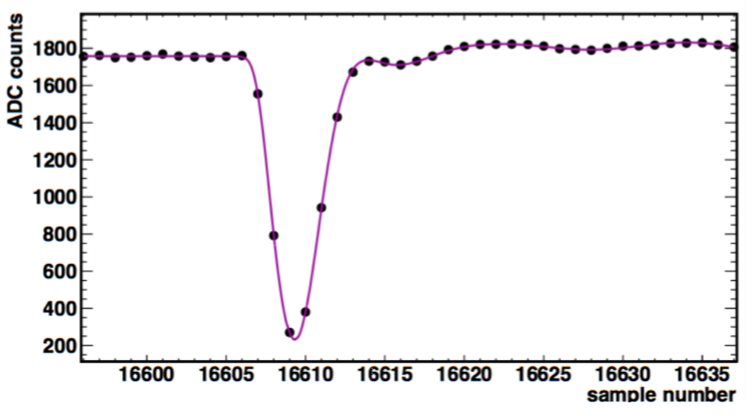
\includegraphics[width=0.6\textwidth]{TemplateFit}
    \caption[Template fit to SiPM trace]{A template fit in purple to a SiPM trace delineated by the black points which is in units of ADC counts. Plot courtesy of Aaron Fienberg.}
    \label{fig:TemplateFit}
\end{figure}


Once a pulse has been fit with a template, the pulse area needs to be converted to real energy units using an energy calibration procedure. A couple of different techniques exist that can be used, including a method that counts photo-statistics seen in the SiPMs \cite{AFThesis}. The default method used is a comparison of lost muon energy signatures in the calorimeters. As described in \refref{lostmuons}, muons lost from the storage ring can spiral inward and hit consecutive calorimeters with a specific time separation between calorimeter hits. These lost muons are minimum-ionizing particles, and thus leave a very distinct energy signature in the crystals, see \secref{sec:lostmuons}. Selecting on the time signature allows hits corresponding to lost muons to be isolated, and the energy signature can be used to determine the appropriate conversions from area to energy\footnote{Different channels can also be equalized based on the energy signatures.}. 


The energy calibration for positron hits as compared to lost muon hits then needs to be determined. Again there are a couple of different techniques, including a comparison of endpoint energies for high energy positrons which tail off at the magic momentum of $\SI{3.094}{\GeV}$, and comparison with simulation. The default technique is to calibrate the energies such that the optimal energy threshold for the \wa analysis is near $\SI{1.7}{\GeV}$ \cite{AFThesis}. Ultimately the energy calibration doesn't matter too much because it is not the energy units that really matter. What really matters is the number of positrons above some energy threshold, where that threshold can be optimized empirically. In fact, the entire \wa analysis could be done without even considering the energy of the incident positrons, and only considering the amplitude of the SiPM pulses\footnote{This statement ignores the effects of pileup which must be accounted for, and applies for a threshold style analysis, and not for other analysis methods which depend on the energy of the pulses.}.


Each pulse fit now has an associated energy and time. Because the measurement of \wa depends heavily on the time reconstruction since the analysis is a frequency extraction, pulse times need to be corrected for various effects in order to reach the precision goal. The fitted times for each pulse need to be aligned on a fill-by-fill basis relative to the injection time of the beam, corrected for any channel differences due to differing pulse shapes or fiber lengths, and corrected for any calorimeter time misalignments due to the use of different laser system components. The fill-by-fill alignment is corrected for using the T0 detector as described in \secref{sec:T0}. The channel differences are corrected by aligning calorimeter channels in time using signals from islands with large simultaneous pulses in neighboring crystals. Calorimeters are time aligned using lost muon coincident events as described before. Once the times of the pulse fits or crystal hits have been determined, the energies can be corrected appropriately for gain effects measured by the laser system. As described in \secref{sub:LaserCalibrationSystem}, the laser calibration system corrects for in-fill, out-of-fill, and SDTP effects \cite{Gain}. \figref{fig:IFGFunction} shows an in-fill gain function fit to data for a single calorimeter. Systematic effects for corrected gain effects are studied in \secref{sub:gainerror}. 

\begin{figure}[]
    \centering
    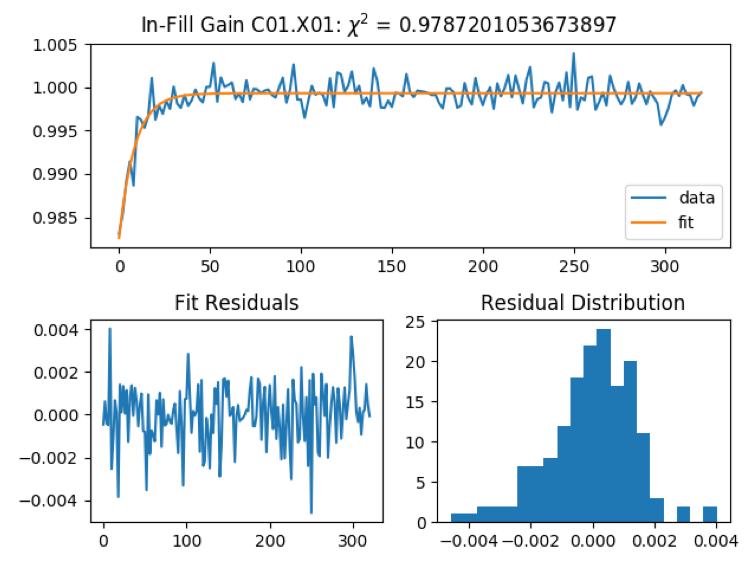
\includegraphics[width=0.6\textwidth]{IFGFunction}
    \caption[In-fill gain function fit for a single calorimeter crystal]{In-fill gain function fit for a single calorimeter crystal (top) and fit residuals (bottom). Each crystal has its own in-fill and SDTP gain function parameters. Plot courtesy of Matthias Smith.}
    \label{fig:IFGFunction}
\end{figure}


The last part of the calorimeter reconstruction is the clustering. Clustering is the stage which takes the individual template fit results from separate crystals, and turns them into the times, energies, and positions of decay positron impacts. For a time island with a single positron impact, the procedure is straightforward. The energy for the positron hit cluster is the sum of the individual hit crystal energies. The time for the cluster is taken as the time of the maximum energy hit in the island. This works because most of the deposited energy from a hit is localized to a single crystal. The position of the cluster is determined with a logarithmic weighting function between crystal hits, which for a $\SI{2}{\GeV}$ positron in the E989 calorimeters results in a resolution of $\SI{2}{mm}$ \cite{AFThesis}. See \figref{fig:CaloCluster} for a single calorimeter cluster from a positron hit in the calorimeter. For a time island with multiple positron impacts, the individual crystal hits are separated in time, where the time partitioning separates hits that are $\SI{2.5}{ns}$ apart, and the clustering proceeds as before. For hits which are within this time window, a pileup event has occurred. If the pileup event happens within the same crystal, then the multiple hits are measured as a single hit, and this needs to be corrected for using a pileup subtraction technique, as described in \secref{sub:pileupsubtraction}. For hits that occur in separate crystals, the pileup can be resolved using the spatial separation of the calorimeters. This is an ongoing area of work, and one technique is described in \refref{AFThesis}. For this analysis the spatial separation was turned off, which simplifies the analysis somewhat. This increases the amount of pileup seen in the data, which then needs to be handled by the pileup subtraction technique. For the precision of the Run 1 analysis result, this was found to be acceptable. 


\begin{figure}[]
    \centering
    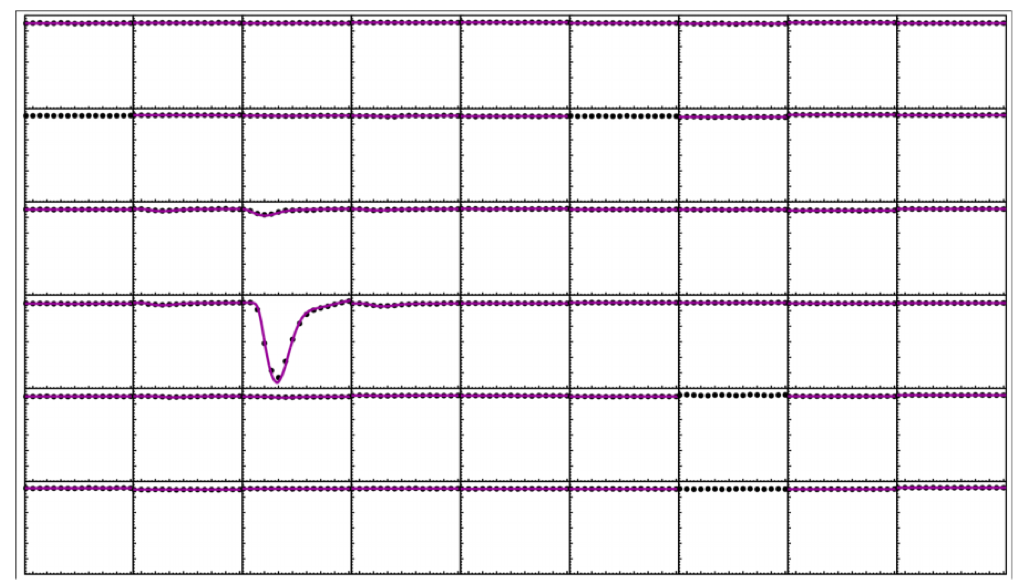
\includegraphics[width=0.9\textwidth]{CaloCluster}
    \caption[Calorimeter cluster from SiPM traces fit with templates]{A single positron hit in the calorimeter, which resulted in a reconstructed calorimeter cluster. Each box is a crystal in the calorimeter, where the contained trace is the SiPM output fit with a template. The positron hit the crystal three from the left and three from the bottom, where it deposited most of its energy. Some of the energy was deposited in the neighboring crystals. Plot courtesy of Aaron Fienberg.}
    \label{fig:CaloCluster}
\end{figure}



\section{Histogramming}
\label{sec:Histogramming}


Once the reconstruction has processed all the hits into clusters, the time spectra histogram needs to be made. First an energy threshold needs to be chosen. As described at the end of \secref{section:WaIntro}, the optimal energy threshold is where the quantity $NA^{2}$ reaches the maximum, at least in the case of a five parameter fit. By scanning over the choice of energy threshold and fitting the resulting time spectra, the optimal energy threshold can be determined as seen in \figref{fig:OptimalEnergyThreshold}. The optimal choice of energy threshold was thus determined to be $\SI{1700}{\MeV}$.





- maybe make some comment about how certain choices in the histogramming were informed by analysis results?


-need a table of chosen parameters in the histogramming - maybe at the end though
-pileup sdt, sgt, adt, energy threshold, others?


    \begin{figure}[]
    \centering
        \begin{subfigure}[t]{0.45\textwidth}
            \centering
            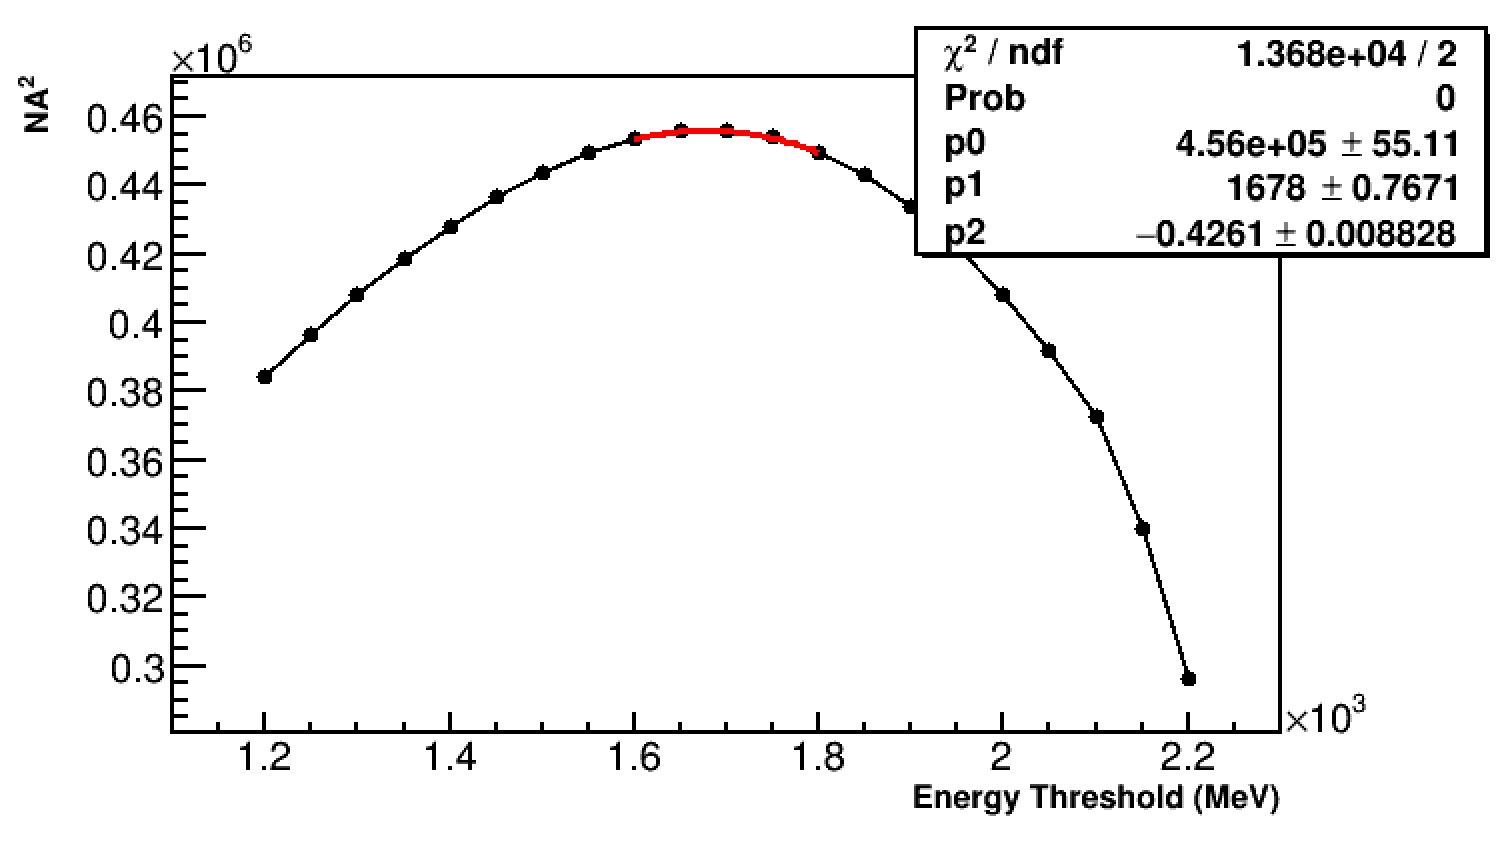
\includegraphics[width=\textwidth]{TemporaryEThresholdNA2}
            \caption{}
        \end{subfigure}
        \begin{subfigure}[t]{0.45\textwidth}
            \centering
            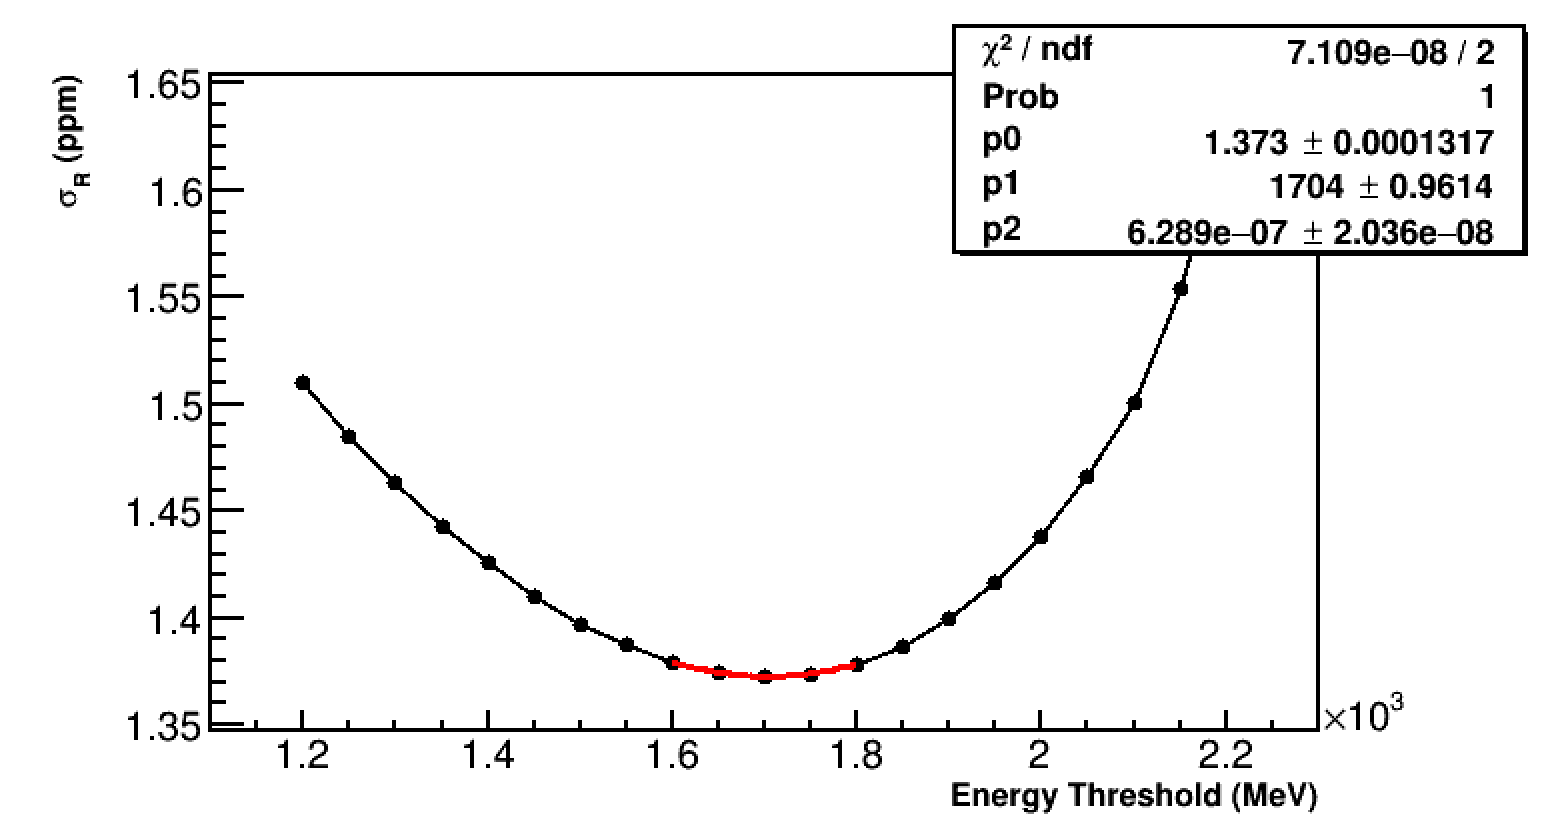
\includegraphics[width=\textwidth]{TemporaryEThresholdRatio}
            \caption{}
        \end{subfigure}% 
    \caption[Determination of optimal energy threshold]{The optimal energy threshold can be determined from the $NA^{2}$ quantity as described in \secref{section:WaIntro} from a five parameter fit to the data (left), or from the calculated error with the final fit function (right). \textbf{temporary energy threshold plots - replace - also not sure how to introduce R and ratio fit stuff here when I haven't talked about it yet}}
    \label{fig:OptimalEnergyThreshold}
    \end{figure}

% \begin{figure}[]
%     \centering
%     % \includegraphics[width=0.9\textwidth]{OptimalEnergyThreshold}
%     \rule{10cm}{10cm}
%     \caption[put caption here]{put a picture of the scanned optimal energy threshold here}
%     \label{fig:OptimalEnergyThreshold}
% \end{figure}




-artificial deadtime - how to talk about this when I have yet to get to pileup method 
-time randomization - at end after application of adt





\subsection{Pileup subtraction}
\label{sub:pileupsubtraction}






\section{Lost muons}
\label{sec:lostmuons}

-need to include delta t plot and energy deposition plot


\cite{lostmuons}




\section{Fitting}
\label{sec:Fitting}




-detail the ratio method - might need to pull stuff out from my appendix


    \begin{figure}[]
    \centering
        \begin{subfigure}[t]{0.45\textwidth}
            \centering
            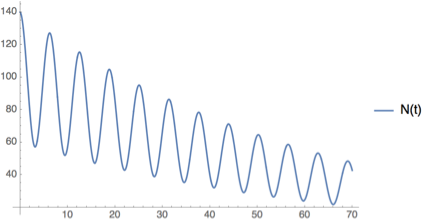
\includegraphics[width=\textwidth]{FiveParamFunc}
            \caption{}
        \end{subfigure}%

        \vspace{2mm}
        \begin{subfigure}[t]{0.45\textwidth}
            \centering
            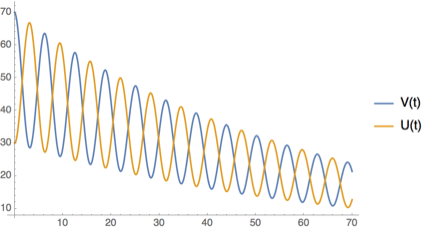
\includegraphics[width=\textwidth]{UVFuncs}
            \caption{}
        \end{subfigure}
        \begin{subfigure}[t]{0.45\textwidth}
            \centering
            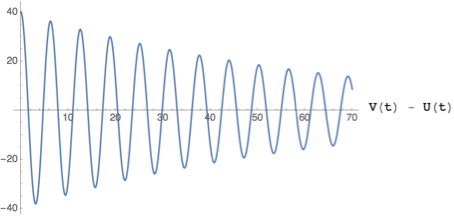
\includegraphics[width=\textwidth]{RatioNumFunc}
            \caption{}
        \end{subfigure}%
        \vspace{2mm}
        \begin{subfigure}[t]{0.45\textwidth}
            \centering
            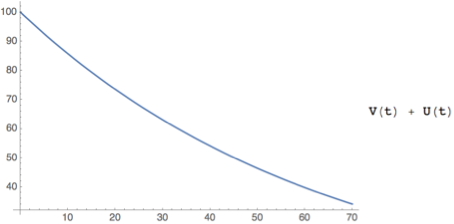
\includegraphics[width=\textwidth]{RatioDenomFunc}
            \caption{}
        \end{subfigure}
        \begin{subfigure}[t]{0.45\textwidth}
            \centering
            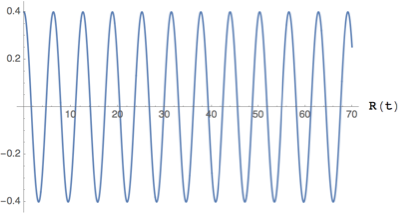
\includegraphics[width=\textwidth]{RatioFunc}
            \caption{}
        \end{subfigure}% 
    \caption[]{}
    \label{}
    \end{figure}


\subsection{CBO terms}
\label{sub:cboterms}






\section{Systematic errors}
\label{sec:Systematic Errors}



\begin{table}[]
\centering
\setlength\tabcolsep{10pt}
\renewcommand{\arraystretch}{1.2}
\begin{tabular*}{.8\linewidth}{@{\extracolsep{\fill}}lc}
  \hline
    \multicolumn{2}{c}{\textbf{\wa Measurement Uncertainties}} \\
  \hline\hline
    Source of uncertainty & E989 Goal (ppb) \\
  \hline
    Gain changes & 20 \\
    Pileup & 40 \\
    Lost muons & 20 \\
    CBO & 30 \\
    E field and pitch corrections & 30 \\
  \hline
    Quadrature sum & 70 \\
  \hline 
\end{tabular*}
\caption[Uncertainties in the precession frequency measurement]{Systematic errors in the precession frequency measurement. \textbf{fill this table out more once I've gone through the various parts}}
\label{tab:wauncertainties}
\end{table}




\subsection{Gain}
\label{sub:gainerror}


-talk about the equations here - slight reference to either detector section or reconstruction section in this chapter



\subsection{Pileup}
\label{sub:pileuperror}


\cleardoublepage
